\documentclass[11pt]{article}
\usepackage[T1]{fontenc}
\usepackage{lmodern}
\usepackage[margin=1in]{geometry}
\usepackage{amsmath,amssymb,amsthm,mathtools}
\usepackage{microtype}
\usepackage{flafter}
\usepackage{tikz}
\usetikzlibrary{arrows.meta,positioning,calc}
\usepackage{xcolor}
\usepackage{xurl}
\usepackage[colorlinks=true,linkcolor=blue!45!black,citecolor=green!35!black,urlcolor=blue!45!black]{hyperref}
\hypersetup{pdftitle={An exponential state lower bound for two-way nondeterministic complementation},pdfauthor={OpenAI},pdfsubject={Alphabet-uniform state complexity of 2NFA complementation}}
\usepackage{enumitem}
\setlist{itemsep=3pt,topsep=5pt}
\newtheorem{theorem}{Theorem}[section]
\newtheorem{lemma}[theorem]{Lemma}
\newtheorem{proposition}[theorem]{Proposition}
\newtheorem{corollary}[theorem]{Corollary}
\theoremstyle{definition}
\newtheorem{definition}[theorem]{Definition}
\theoremstyle{remark}
\newtheorem{remark}[theorem]{Remark}
\numberwithin{equation}{section}
\title{An exponential state lower bound for\newline two-way nondeterministic complementation}
\author{OpenAI}
\date{September 25, 2026}
\begin{document}
\maketitle
\begin{abstract}
We prove that two-way nondeterministic finite automata cannot be
complemented with a polynomial number of states independent of the
alphabet. For each $n\ge4$ we construct an $n$-state automaton over a finite
alphabet whose complement requires at least
$\tfrac12 2^{\lfloor(n-4)/127\rfloor}-1$ states.
\end{abstract}
\section{Introduction}
\label{sec:introduction}

A two-way nondeterministic finite automaton (2NFA) has a finite set of
states and a single read-only head, which may move in either direction
along an input bounded by endmarkers. It accepts when some finite
computation reaches an accepting state. The complementation problem asks
whether every $n$-state 2NFA over a finite alphabet $\Sigma$ has a 2NFA for
the complementary language with at most $p(n)$ states, for one polynomial
$p$ independent of $\Sigma$. We answer this question negatively.

For exact state counts, there is one initial state and a set of accepting
states. Each transition depends only on the current state and scanned
symbol, updates the state, and moves the head left, right, or not at all.
We start the head on the left endmarker and forbid moves beyond either
endmarker. Missing transitions
reject that branch; infinite nonaccepting computations do not accept.
An accepting initial configuration counts as acceptance. All states,
including initial and accepting states, are counted. A deterministic
two-way automaton (2DFA) has at most one successor for each state and
scanned symbol.

For a finite set $H$, let $\mathcal R_H$ denote all binary relations on
$H$. Products are composed in path order:
$(p,r)\in AB$ if and only if $(p,q)\in A$ and $(q,r)\in B$ for some $q$.
Use $\Sigma_H=\mathcal R_H$ as an input alphabet. The product $r(w)$ of a
word $w=R_1\cdots R_k$ is $R_1\cdots R_k$, and the empty product is
$r(\varepsilon)=I_H=\{(p,p):p\in H\}$. Define the relation-product
liveness language
\[
 L_H=\{w\in\Sigma_H^*:r(w)\ne\varnothing\}.
\]
In particular, $L_H$ contains the empty word when $H$ is nonempty.
For nonempty words, this is Sakoda and Sipser's family $B_h$, where
$h=|H|$ \cite[Section~2.1 and Theorem~2.3]{SakodaSipser1978}; the name
\emph{one-way liveness} is used in \cite[Section~2.2]{Kapoutsis2006}.

\begin{theorem}\label{main:theorem}
For every integer $n\ge4$, set $H=\{1,\ldots,n-2\}$ and
$\Sigma_n=\mathcal R_H$. There is an $n$-state 2NFA $A_n$ recognizing
$L_H$ such that every 2NFA recognizing
$\Sigma_n^*\setminus L(A_n)$ has at least
\[
 \frac12\,2^{\lfloor(n-4)/127\rfloor}-1
\]
states. In particular, there is no polynomial state bound for
complementation that is independent of the finite alphabet.
\end{theorem}

The alphabet $\Sigma_n$ consists of all binary relations on a set of
$n-2$ points, so $|\Sigma_n|=2^{(n-2)^2}$. The parameter is the
number of states, not the size of the transition table. Theorem~\ref{main:theorem}
concerns bounds uniform over finite alphabets; it does not assert a lower
bound over one fixed alphabet.

\paragraph{History and significance.}
Sakoda and Sipser's work on nondeterminism and two-way finite automata
\cite{SakodaSipser1978} initiated the central state-succinctness problem of
simulating two-way nondeterministic automata deterministically.
Complementation is a separate question: here the target remains
nondeterministic. Vardi's construction gives an exponential-state
one-way nondeterministic automaton for the complement of a two-way
nondeterministic automaton \cite[Theorem~3.2]{Vardi1989}. It certifies
nonacceptance by locally consistent sets of states. For sweeping
automata, whose head can reverse direction only at the endmarkers,
Kapoutsis proved that the complement of one-way liveness requires
exponentially many states in every sweeping 2NFA
\cite[Theorem~1]{Kapoutsis2006}. Theorem~\ref{main:theorem}
allows unrestricted two-way motion in the complementing automaton.

For deterministic two-way automata, complementation
has a linear state bound independent of the alphabet
\cite{GeffertMereghettiPighizzini2007}.
Guillon, Prigioniero, and Taheri describe polynomial 2NFA
complementation as open \cite[Section~1]{GuillonPrigionieroTaheri2026}
and give polynomial complementation by 1-limited automata
\cite[Theorem~4.1]{GuillonPrigionieroTaheri2026}. These automata may
rewrite a tape cell on its first visit; this resource is absent from
the read-only model considered here.
Theorem~\ref{main:theorem} resolves the alphabet-uniform polynomial
complementation question negatively. The same growing-alphabet family
also requires exponentially many states in every equivalent deterministic
two-way automaton: a smaller deterministic simulator could be
complemented with linear state overhead. Corollary~\ref{auto:determinization}
makes this implication explicit, including the treatment of infinite
nonaccepting computations.

The companion paper \cite[Theorem~1.1]{CompanionDeterminization2026}
proves a deterministic lower bound with a larger exponential rate for the
same language, by an independent matching-diagram argument. We compare
the exact bounds after Corollary~\ref{auto:determinization}. The new
obstruction here applies even when the complementing machine is
nondeterministic.

\paragraph{The argument.}
An automaton with $h+2$ states guesses a path through the
relations and accepts exactly when their product is nonempty.
We prove that recognizing product emptiness requires exponentially many
states.

The proof separates a representation of computations from a finite
algebraic lower bound. A segment of a computation is represented by four
relations recording the possible entries and exits through its two
boundaries. These \emph{path diagrams} compose by joining boundaries.
Their monoid is the monoid of partitioned binary relations introduced
by Martin and Mazorchuk \cite[Sections~2.1--2.3]{MartinMazorchuk2013},
written with separate labels for the two directions of travel.
Adding edges only increases the available accepting paths. On the other
hand, singleton relation contexts test the absence of any prescribed
pair. Consequently a machine for product emptiness induces a
surjective multiplicative map from its path diagrams to the relation
monoid that reverses inclusion.

To bound such maps, we attach recurrent classes of boundary labels to an
idempotent diagram $e$, meaning $e^2=e$. These classes group labels joined
in both directions by through paths together with returns. Their precise
definition is given in Section~\ref{sec:diagrams}.
The diagrams $z$ satisfying $ez=ze=z$ form a
submonoid with identity $e$, called its \emph{corner}. Such a $z$ may
destroy the loops on some of those classes; we record the destroyed
classes as a missing set. Two structural facts
control this loss. First, one common missing-set bound transports through
any fixed diagram context with only a factor of two. Second, along a
chain of nested idempotents the sum of successive losses is bounded by
twice a single initial missing-set budget. The second fact permits the
corner identity to change during the argument.

For an integer parameter $t$, the amplification step converts $2t$
conjugates of one relation with an added off-diagonal pair
into $t^2$ additions sharing a common budget. Each addition, after
restriction to a smaller relation corner, incurs an inductively bounded
loss. Taking $t=64$ gives the exponential recurrence. This strategy
adapts the conjugate-amplification pattern of the matching-diagram
rank-loss argument in
\cite[Section~3]{CompanionDeterminization2026}; that argument concerns a deterministic
state lower bound. Here all diagram paths may be nondeterministic, and
the transport and nested-class bounds are proved anew. They are stated
independently of automata and may be useful for other order-reversing
images of finite path monoids.

Section~\ref{sec:diagrams} states the algebraic bound and derives the
order-reversing map before developing recurrent classes and transport.
Section~\ref{nest:section} proves the chain bound, and
Section~\ref{amp:section} proves the algebraic lower bound.
Section~\ref{auto:section} proves the promised automata representation and
completes the proof of Theorem~\ref{main:theorem}.

The bounds impose no restriction on input length or on the running time
of a successful computation. They compare finite-state machines without
a work tape, and give no separation between uniform logarithmic-space
complexity classes.

\section{Path diagrams and missing recurrent classes}
\label{sec:diagrams}

We first describe finite paths through a segment, without assuming that
the paths come from an automaton. Our goal is a loss measure that detects
edge inclusion and remains controlled when a segment is put in context.

Relations are composed in \emph{path order}: $x(AB)y$ means that
$xAz$ and $zBy$ for some $z$. On a single set, $A^*$ denotes the reflexive
transitive closure, so it includes paths of length zero. We use the
elementary path identities
\begin{equation}\label{diag:star}
 (A\cup B)^*=A^*(BA^*)^*,\qquad
 A(BA)^*=(AB)^*A.
\end{equation}
The first groups successive $A$-steps between $B$-steps; the second groups
the same alternating path from its opposite end. These identities hold
whenever the relation types permit the displayed products.

\subsection{The diagram monoid}

Fix disjoint sets $D^+$ and $D^-$, each of size $m\ge1$.
A diagram $a$ consists of four arbitrary relations
\[
 F_a\subseteq D^+\times D^+,\quad
 B_a\subseteq D^-\times D^-,\quad
 L_a\subseteq D^+\times D^-,\quad
 R_a\subseteq D^-\times D^+.
\]
Entering the segment on the left uses a label of $D^+$; $F_a$ records an
exit on the right and $L_a$ an exit on the left. Entering on the right uses
a label of $D^-$; $B_a$ records an exit on the left and $R_a$ an exit on
the right. The relations $F_a,B_a$ are the \emph{through relations}, and
$L_a,R_a$ are the \emph{return relations}; see Figure~\ref{fig:diagram}.

\begin{figure}[tb]
\centering
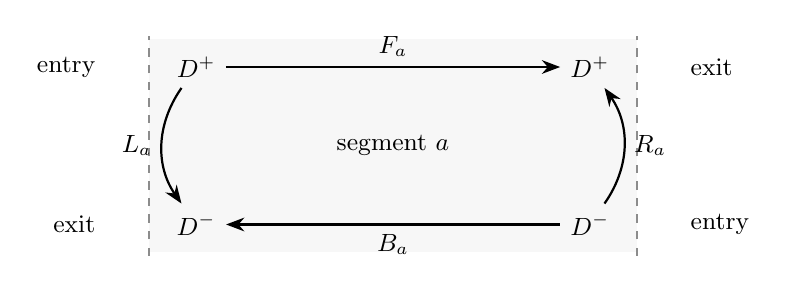
\begin{tikzpicture}[>=Stealth,thick,font=\small]
 \fill[black!3] (0.4,-0.35) rectangle (6.6,2.35);
 \draw[dashed,black!45] (0.4,-0.4)--(0.4,2.4);
 \draw[dashed,black!45] (6.6,-0.4)--(6.6,2.4);
 \node (lp) at (1,2) {$D^+$};
 \node (lm) at (1,0) {$D^-$};
 \node (rp) at (6,2) {$D^+$};
 \node (rm) at (6,0) {$D^-$};
 \draw[->] (lp)--node[above] {$F_a$}(rp);
 \draw[->] (rm)--node[below] {$B_a$}(lm);
 \draw[->] (lp) to[bend right=35] node[left] {$L_a$}(lm);
 \draw[->] (rm) to[bend right=35] node[right] {$R_a$}(rp);
 \node at (3.5,1) {segment $a$};
 \node[anchor=east] at (-0.15,2) {entry};
 \node[anchor=east] at (-0.15,0) {exit};
 \node[anchor=west] at (7.15,2) {exit};
 \node[anchor=west] at (7.15,0) {entry};
\end{tikzpicture}
\caption{The four relations of a path diagram. Each arrow represents a
relation between entire label sets, not a single deterministic edge.
In a product, an exit enters the neighboring segment with the same label.}
\label{fig:diagram}
\end{figure}

Place diagrams in a line. At each internal boundary, identify an exit
with the entry of the neighboring diagram bearing the same label.
The product records finite paths from an outer entry to the first outer
exit, with all earlier joins internal. A traversal of any consecutive
block can be replaced by one edge of the block's product, and that edge
can conversely be expanded into a finite traversal. This proves
associativity. The diagram with $F$ and $B$ identity relations and $L,R$
empty is the identity. Thus the diagrams form a finite monoid
$\mathcal T_m$.

This is the degree-$m$ monoid of partitioned binary relations of
Martin and Mazorchuk \cite[Sections~2.1--2.3]{MartinMazorchuk2013}.
To identify the two descriptions, label $D^+$ and $D^-$ by a common
$m$-element set. At each boundary, an entry and an exit with the same
underlying label give one vertex. The four relations above become
the four blocks of a binary relation on the left and right vertex
sets. A join always switches from one factor to its neighbor, exactly
as in their alternating-path composition. We have included the
path expansion and contraction proof of associativity to fix the
finite-path convention used below.

Write $a\sqsubseteq b$ when all four relations of $a$ are included in
the corresponding relations of $b$. Products preserve this order in
each argument. Joining two diagrams at one boundary gives
\begin{equation}\label{diag:product}
\begin{aligned}
 F_{ab}&=F_a(L_bR_a)^*F_b,&
 B_{ab}&=B_b(R_aL_b)^*B_a,\\
 L_{ab}&=L_a\cup F_a(L_bR_a)^*L_bB_a,&
 R_{ab}&=R_b\cup B_bR_a(L_bR_a)^*F_b.
\end{aligned}
\end{equation}
For example, a forward path crosses $a$, alternates returns at the join,
and crosses $b$. Reflection exchanges $D^+$ with $D^-$, $F$ with $B$,
and $L$ with $R$, while reversing product order. We will prove symmetric
statements for the positive sign and obtain the negative sign by this
reflection.

\subsection{From complementation to an order-reversing image}

The algebraic obstruction to complementation is the following bound.
As in the introduction, $\mathcal R_H$ is the monoid of all binary
relations on $H$, composed in path order.

\begin{theorem}[Order-reversing image bound]
\label{amp:image}
\label{amp:relation-bound}
Let $m\geq1$, let $H$ be a finite set of cardinality $h\geq2$, and let
$S_0$ be a submonoid of $\mathcal T_m$.  Suppose that a surjective
multiplicative map $\phi_0:S_0\to\mathcal R_H$ satisfies
\begin{equation}
 z\sqsubseteq w\quad\Longrightarrow\quad
 \phi_0(w)\subseteq\phi_0(z)
 \qquad(z,w\in S_0).
 \label{amp:reverse}
\end{equation}
Then
\begin{equation}
 2m\geq 2^{\lfloor(h-2)/127\rfloor}.
 \label{amp:bound}
\end{equation}
The map need not initially be assumed to preserve identities.
\end{theorem}

The proof is completed in Section~\ref{amp:section}. We first explain
the automata reduction, using the finite-computation representation
below. Its construction, proved in
Section~\ref{auto:finite-computations}, uses one additional state to
represent success by an exit past the right endmarker. Local diagram
edges record finitely many stay moves followed by one move out of a
cell; no bound on repeated crossings is imposed.

\begin{lemma}\label{auto:representation}
Let $B$ be an $s$-state 2NFA over a finite alphabet $\Sigma$ in the model
fixed in the introduction. There are a monoid homomorphism
\[
  \tau:\Sigma^*\longrightarrow\mathcal T_{s+1},
\]
two fixed endmarker diagrams $\lambda,\rho\in\mathcal T_{s+1}$,
and fixed positive labels $a,b$ such that, for every word $w$,
\begin{equation}\label{auto:recognition}
  w\in L(B)
  \quad\Longleftrightarrow\quad
  (a,b)\in F_{\lambda\tau(w)\rho}.
\end{equation}
Consequently, if $\tau(u)\sqsubseteq\tau(v)$, then
\begin{equation}\label{auto:context-monotonicity}
  \alpha u\beta\in L(B)
  \quad\Longrightarrow\quad
  \alpha v\beta\in L(B)
  \qquad(\alpha,\beta\in\Sigma^*).
\end{equation}
\end{lemma}
The acceptance equivalence immediately implies the stated monotonicity
in arbitrary word contexts:
\begin{proof}[Derivation of context monotonicity]
Diagram multiplication is increasing in each factor.
If $\tau(u)\sqsubseteq\tau(v)$, then
\[
 \lambda\tau(\alpha)\tau(u)\tau(\beta)\rho
 \ \sqsubseteq\
 \lambda\tau(\alpha)\tau(v)\tau(\beta)\rho.
\]
The designated forward edge persists under this inclusion.  Applying
\eqref{auto:recognition} proves
\eqref{auto:context-monotonicity}.
\end{proof}

For relation-product emptiness, singleton contexts convert this
increasing behavior of acceptance into a decreasing relation image.
For $F\subseteq H$, write $I_F=\{(x,x):x\in F\}$.
A multiplicative map is \emph{unital} if it preserves identities.

\begin{proposition}\label{auto:order-reversal}
Let $H$ be a finite set with at least two elements. If an $s$-state
2NFA recognizes $\Sigma_H^*\setminus L_H$, then a
submonoid of $\mathcal T_{s+1}$ admits a surjective unital
homomorphism $\phi$ onto $\mathcal R_H$ satisfying
\begin{equation}\label{auto:reverse-order}
  z\sqsubseteq z'
  \quad\Longrightarrow\quad
  \phi(z')\subseteq\phi(z).
\end{equation}
\end{proposition}
\begin{proof}
Apply Lemma~\ref{auto:representation} to the complementing machine,
and let $S=\tau(\Sigma_H^*)$.  Suppose
$\tau(u)\sqsubseteq\tau(v)$.  For each $p,q\in H$, take the
one-letter words
\[
  \alpha=I_{\{p\}},\qquad \beta=I_{\{q\}}.
\]
They belong to $\Sigma_H$, and
\[
 I_{\{p\}}r(u)I_{\{q\}}
 =
 \begin{cases}
   \{(p,q)\},& (p,q)\in r(u),\\
   \varnothing,&(p,q)\notin r(u).
 \end{cases}
\]
Since the machine accepts exactly the words with empty relation
product, \eqref{auto:context-monotonicity} implies
\[
  (p,q)\notin r(u)
  \quad\Longrightarrow\quad
  (p,q)\notin r(v).
\]
Thus
\begin{equation}\label{auto:word-order}
  \tau(u)\sqsubseteq\tau(v)
  \quad\Longrightarrow\quad
  r(v)\subseteq r(u).
\end{equation}

If $\tau(u)=\tau(v)$, applying \eqref{auto:word-order} in both
directions yields $r(u)=r(v)$.  Therefore
\[
  \phi:S\longrightarrow\mathcal R_H,
  \qquad \phi(\tau(w))=r(w),
\]
is well-defined.  Concatenation of words proves multiplicativity, and
the empty word proves preservation of the identity.  It is surjective
because every relation in $\mathcal R_H$ is itself a letter of
$\Sigma_H$.  Equation~\eqref{auto:word-order} is exactly the required
order reversal \eqref{auto:reverse-order}.
\end{proof}

With $m=s+1$, Theorem~\ref{amp:image} therefore bounds the states of a
complementing machine. Section~\ref{auto:section} constructs the
$h+2$-state source machine and completes the numerical deduction.
It remains to prove the algebraic bound. The next subsection associates
at most $2m$ recurrent classes with an idempotent diagram. We will measure
loss by the classes whose through loops are missing, and force that
loss to grow exponentially with $h$.

\subsection{Recurrent classes in a corner}

For an idempotent $e\in\mathcal T_m$, define
\begin{equation}\label{diag:KP}
\begin{aligned}
 K_e^+&=(L_eR_e)^*,& P_e^+&=K_e^+F_eK_e^+,\\
 K_e^-&=(R_eL_e)^*,& P_e^-&=K_e^-B_eK_e^-.
\end{aligned}
\end{equation}
When working only with the positive sign we omit superscripts.
By $e^2=e$ and \eqref{diag:product},
\begin{equation}\label{diag:idempotent}
 F_eK_eF_e=F_e,\qquad P_e^2=P_e.
\end{equation}
In particular, $P_e$ is transitive. A point $x\in D^\sigma$ is
\emph{recurrent} if $xP_e^\sigma x$. Mutual relatedness under
$P_e^\sigma$ is an equivalence relation on the recurrent points.
Let $\mathcal C_e$ be the collection of its classes for both signs,
keeping the signs distinct. Then
\begin{equation}\label{diag:class-count}
 |\mathcal C_e|\le2m.
\end{equation}
For the identity diagram, $K_e^\sigma=P_e^\sigma$ is the identity
relation on $D^\sigma$, so all $2m$ directional labels form singleton
recurrent classes.

The \emph{corner} $e\mathcal T_me=\{eae:a\in\mathcal T_m\}$ is a monoid
with identity $e$; membership is equivalent to $ez=ze=z$.
For $z$ in this corner put
\[
 U_e^+(z)=K_e^+F_zK_e^+,\qquad
 U_e^-(z)=K_e^-B_zK_e^-.
\]
The return formulas and the two corner identities give
\begin{equation}\label{diag:corner}
 L_e\subseteq L_z,\quad R_e\subseteq R_z,\qquad
 F_z=F_e(L_zR_e)^*F_z=F_z(L_eR_z)^*F_e.
\end{equation}
Consequently
\begin{equation}\label{diag:corner-absorb}
 F_eK_eF_z\subseteq F_z,\quad F_zK_eF_e\subseteq F_z,
 \qquad P_eU_e(z),\ U_e(z)P_e\subseteq U_e(z).
\end{equation}
The last two inclusions follow by multiplying the first two by $K_e$
on the appropriate sides. If $x,y$ belong to one recurrent class, then
$yP_ex$, $xP_ey$, and \eqref{diag:corner-absorb} show that a loop
$xU_e(z)x$ implies $yU_e(z)y$. Reflection gives the same fact for the
negative sign. Hence the following is well-defined:
\[
 \mathcal M_e(z)=\{C\in\mathcal C_e:
       xU_e^\sigma(z)x\text{ fails for }x\in C,
       \text{ where }C\subseteq D^\sigma\}.
\]
We call $\mathcal M_e(z)$ the \emph{missing set} of $z$ relative to $e$.

\begin{lemma}[Products of missing sets]\label{diag:missing}
Let $e\in\mathcal T_m$ be idempotent. For $z,w\in e\mathcal T_me$,
\[
 \mathcal M_e(zw)\subseteq\mathcal M_e(z)\cup\mathcal M_e(w),
 \qquad \mathcal M_e(e)=\varnothing.
\]
In particular, $\mathcal M_e(z^k)\subseteq\mathcal M_e(z)$ for every
positive integer $k$.
\end{lemma}
\begin{proof}
The returns of $e$ persist in both $z$ and $w$, so
$(L_wR_z)^*\supseteq K_e$. Formula~\eqref{diag:product} therefore gives
$U_e^+(zw)\supseteq U_e^+(z)U_e^+(w)$. Two loops at the same point
compose to a loop. For the negative sign the corresponding product is
$U_e^-(w)U_e^-(z)$, which gives the same conclusion. Finally
$U_e^\sigma(e)=P_e^\sigma$, so no recurrent class is missing from $e$.
\end{proof}

\begin{lemma}[Rectangles of through edges]\label{diag:rectangles}
Let $e\in\mathcal T_m$ be idempotent and let $z\in e\mathcal T_me$.
For a positive recurrent class $C\in\mathcal C_e$ and any $p\in C$, set
\[
 A_C=\{u:u(F_eK_e)p\},\qquad
 B_C=\{v:p(K_eF_e)v\}.
\]
The rectangle $A_C\times B_C$ is independent of $p$ and is contained
in $F_e$. These rectangles cover $F_e$. If
$C\notin\mathcal M_e(z)$, its rectangle is contained in $F_z$.
The reflected assertions hold for negative classes and $B_e$.
In particular,
\begin{equation}\label{diag:detect}
 \mathcal M_e(z)=\varnothing\quad\Longrightarrow\quad e\sqsubseteq z.
\end{equation}
\end{lemma}
\begin{proof}
Containment in $F_e$ follows from $F_eK_eF_e=F_e$.
The identities
\[
 (F_eK_e)P_e=F_eK_e,\qquad P_e(K_eF_e)=K_eF_e
\]
show that replacing $p$ by a mutually $P_e$-related point does not
change either factor of the rectangle.

To prove coverage, \eqref{diag:idempotent} implies
$F_eP_e^kF_e=F_e$ for every $k\ge1$. Given a pair in $F_e$, choose a
witness for this expression with $k>m$. Some label repeats along the
$P_e$ portion. That label $p$ is recurrent, since a nonempty $P_e$-path
from $p$ back to itself is a $P_e$-edge by transitivity. The portions
before and after $p$ belong to $F_eK_e$ and $K_eF_e$: indeed
$F_eP_e^j\subseteq F_eK_e$ and $P_e^jF_e\subseteq K_eF_e$ for
$j\ge0$, including $j=0$ since $K_e$ is reflexive.

If $C$ is not missing from $z$, insert $pK_eF_zK_ep$ between the two
halves of its rectangle. The resulting relation is contained in
$F_eK_eF_zK_eF_e\subseteq F_z$ by
\eqref{diag:corner-absorb}. Reflection proves the backward assertion.
When the missing set is empty all through edges of $e$ are thus present
in $z$, and its return edges persist by \eqref{diag:corner}.
\end{proof}

\subsection{Transport through a fixed context}

The next statement controls a whole family of replacements at once.
The common target set, rather than merely a bound for each replacement,
will be essential in the amplification argument.

\begin{lemma}[Transport]\label{diag:transport}
Let $e,d\in\mathcal T_m$ be idempotents and let $u,v\in\mathcal T_m$
satisfy $uev=d$. For every $J\subseteq\mathcal C_e$ there exists a single
set $J'\subseteq\mathcal C_d$, with $|J'|\le2|J|$, such that
\[
 \mathcal M_d(uzv)\subseteq J'
\]
for every $z\in e\mathcal T_me$ satisfying
$\mathcal M_e(z)\subseteq J$ and $uzv\in d\mathcal T_md$.
\end{lemma}
\begin{proof}
For each positive class of $\mathcal C_d$, choose a representative $x$
and a witness for $xK_d^+F_{uev}K_d^+x$. Expand the middle edge into an
actual finite path through the three diagrams $u,e,v$. For a negative
class do the same with $xK_d^-B_{uev}K_d^-x$. Make these choices once,
independently of $z$.

For every occurrence of a through edge of the middle factor $e$ on a
chosen path, choose an $e$-class whose rectangle covers that edge, using
Lemma~\ref{diag:rectangles}. Mark a $d$-class if any class chosen along
its witness lies in $J$; let $J'$ be the marked set. If a class is
unmarked, all its chosen through edges survive replacement of $e$ by
$z$, as do all return edges of $e$. Its original outer $K_d^\sigma$
pieces remain fixed. Thus its witness is a loop in $U_d^\sigma(uzv)$,
and the class is not missing. This proves the required common-set
inclusion.

It remains to count marked classes. For each $d$-class $C$, let $S_C$
be the set of $e$-classes chosen along its fixed witness. We show that
the sets $S_C$ are pairwise disjoint among $d$-classes of a fixed sign.
Consider two positive witnesses, written as
\[
 xK_d^+\alpha\;F_d\;\beta K_d^+x,
 \qquad yK_d^+\alpha'\;F_d\;\beta'K_d^+y,
\]
where $\alpha,\beta,\alpha',\beta'\in D^+$ and the displayed
$F_d$-edges have been expanded through $u,e,v$.
Suppose the expanded paths use occurrences of middle-factor edges
$(a,b)$ and $(a',b')$ covered by one $e$-class. Its rectangle also
contains $(a,b')$ and $(a',b)$. The sign of that $e$-class fixes the
orientation of both edges and their entry and exit boundaries inside
the three-factor product. Thus the prefix ending at $a$, the crossed
edge $(a,b')$, and the suffix starting at $b'$ concatenate to a path
from $\alpha$ to $\beta'$. Neither retained subpath has an earlier
outer exit. The concatenation is therefore a valid finite path for
$F_d$, even if it repeats internal crossings or its selected middle
edge points backward. Interchanging the two prefixes and suffixes
similarly gives $\alpha'F_d\beta$.

The original exterior factors now give $xP_d^+y$ and $yP_d^+x$, so
$x$ and $y$ belong to the same recurrent class. Reflection gives the
same conclusion for negative witnesses, with $B_d$ in place of $F_d$.
This proves the asserted disjointness for each sign. A witness using
only returns of $e$ has $S_C=\varnothing$ and is never marked. Since
$J'=\{C:S_C\cap J\ne\varnothing\}$, at most $|J|$ classes of each
sign are marked, and $|J'|\le2|J|$.
\end{proof}

\section{A loss budget for nested idempotents}
\label{nest:section}

For idempotents in a semigroup, write $d\trianglelefteq e$ if
$de=ed=d$, and say that $d$ is \emph{nested under} $e$.
This is a partial order: reflexivity and antisymmetry are immediate,
and if $d\trianglelefteq e\trianglelefteq f$, then
$df=(de)f=d(ef)=de=d$ and $fd=f(ed)=(fe)d=ed=d$.
Nesting is distinct from the edge-inclusion order $\sqsubseteq$.

We will bound the sum of the losses incurred along a nested chain,
even though the identity, the recurrent classes, and hence the meaning
of a loss change at every step. The key fact is a containment dichotomy:
a new recurrent class contains either an old class that is not lost,
or at least two old classes.

\begin{lemma}[Absorption under nesting]
\label{nest:absorption}
Let $d,e\in\mathcal T_m$ be idempotents with $d\trianglelefteq e$.
For either sign $\sigma$,
\[
 K_e^\sigma\subseteq K_d^\sigma,
 \qquad
 P_e^\sigma P_d^\sigma\subseteq P_d^\sigma,
 \qquad
 P_d^\sigma P_e^\sigma\subseteq P_d^\sigma.
\]
In the positive sign one also has
\begin{equation}
\label{nest:through-absorption}
 F_eP_d^+\subseteq P_d^+,
 \qquad P_d^+F_e\subseteq P_d^+.
\end{equation}
The corresponding negative-sign inclusions use $B_e$.
\end{lemma}

\begin{proof}
We prove the positive-sign statements and suppress the superscript $+$.
Because $d\in e\mathcal T_m e$, its returns contain those of $e$:
$L_e\subseteq L_d$ and $R_e\subseteq R_d$.
Set
\[
 S=(L_dR_e)^*,\qquad T=(L_eR_d)^*.
\]
Then $K_e\subseteq S,T\subseteq K_d$.
The multiplication formulas applied to $ed=de=d$ give
\begin{align}
 F_d&=F_eSF_d=F_dTF_e,\label{nest:forward-identities}\\
 L_d&=L_e\cup F_eSL_dB_e,
 &R_d&=R_e\cup B_eR_dTF_e.
 \label{nest:return-identities}
\end{align}

We spell out the two star rearrangements needed below, using the
finite-path identities in \eqref{diag:star}.
Expanding $R_d$ in $K_d=(L_dR_d)^*$, we obtain
\begin{align*}
 K_d
 &=\bigl(L_dR_e\cup L_dB_eR_dTF_e\bigr)^*\\
 &=S\bigl(L_dB_eR_dTF_eS\bigr)^*,\\
 F_eK_dF_d
 &=\bigl(F_eSL_dB_eR_dT\bigr)^*F_eSF_d\\
 &=\bigl(F_eSL_dB_eR_dT\bigr)^*F_d
 \subseteq K_dF_d.
\end{align*}
Indeed, $F_eSL_dB_e\subseteq L_d$ by
\eqref{nest:return-identities}, so the relation inside the last star
is contained in $L_dR_dT\subseteq K_d$.
For the other side, expand $L_d$ instead:
\begin{align*}
 K_d
 &=\bigl(L_eR_d\cup F_eSL_dB_eR_d\bigr)^*\\
 &=T\bigl(F_eSL_dB_eR_dT\bigr)^*,\\
 F_dK_dF_e
 &=F_dTF_e\bigl(SL_dB_eR_dTF_e\bigr)^*\\
 &=F_d\bigl(SL_dB_eR_dTF_e\bigr)^*
 \subseteq F_dK_d.
\end{align*}
Here $B_eR_dTF_e\subseteq R_d$, so the relation inside the star
is contained in $SL_dR_d\subseteq K_d$.
These inclusions, multiplied by the remaining $K_d$, prove
\eqref{nest:through-absorption} because $P_d=K_dF_dK_d$.
Finally, $K_dP_d=P_dK_d=P_d$ and $K_e\subseteq K_d$ imply
\[
 P_eP_d=K_eF_eK_eP_d\subseteq P_d,
 \qquad P_dP_e=P_dK_eF_eK_e\subseteq P_d.
\]
Reflection proves all negative-sign statements.
\end{proof}

\begin{lemma}[Containment of recurrent classes]
\label{nest:containment}
Let $d,e\in\mathcal T_m$ be idempotents with $d\trianglelefteq e$.
Every class in $\mathcal C_d$ contains either
\begin{enumerate}
 \item a whole class in $\mathcal C_e\setminus\mathcal M_e(d)$; or
 \item two distinct whole classes in $\mathcal C_e$.
\end{enumerate}
All classes in either containment have the same sign.
\end{lemma}

\begin{proof}
Again work in the positive sign and omit its superscript.
Fix a recurrent point $x$ of $P_d$.
Using \eqref{nest:forward-identities} twice, its recurrence gives
\[
 x\bigl(K_dF_eSF_dTF_eK_d\bigr)x.
\]
By the rectangle cover in Lemma~\ref{diag:rectangles}, each of the
two displayed $F_e$-edges can be factored through an $e$-recurrent
point. Denote the first point by $p$ and the second by $q$.
The resulting witness has the form
\begin{equation}
\label{nest:factored-witness}
 x\,\alpha\,p\,\beta\,q\,\gamma\,x,
\end{equation}
where
\begin{align*}
 \alpha&=K_dF_eK_e,\\
 \beta&=K_eF_eSF_dTF_eK_e=K_eF_dK_e=U_e^+(d),\\
 \gamma&=K_eF_eK_d.
\end{align*}
Here $\beta\subseteq P_d$ because $K_e\subseteq K_d$.
Moreover, Lemma~\ref{nest:absorption} shows that multiplying $P_d$
on either side by $\alpha$ or $\gamma$ gives a subrelation of $P_d$.
Thus all four endpoint relations needed for class membership follow
from \eqref{nest:factored-witness} and $xP_dx$:
\[
\begin{array}{ll}
 x\,P_d\,x\,\alpha\,p &\Longrightarrow xP_dp,\\
 p\,\beta\,q\,\gamma\,x &\Longrightarrow pP_dx,\\
 x\,\alpha\,p\,\beta\,q &\Longrightarrow xP_dq,\\
 q\,\gamma\,x\,P_d\,x &\Longrightarrow qP_dx.
\end{array}
\]
In particular $p$ and $q$ are recurrent for $P_d$ and belong to the
class of $x$. In the first and last lines, inserting the recurrence
at $x$ is essential: the shorter witness portion alone need not
contain a $d$-through edge.

The entire $P_e$-class of $p$ lies in the $P_d$-class of $x$.
Indeed, if $r$ is in the former class, then
$xP_dpP_er$ and $rP_epP_dx$, and the two mixed absorptions of
Lemma~\ref{nest:absorption} give $xP_dr$ and $rP_dx$.
The same argument applies to $q$.
If their $P_e$-classes are distinct, this proves the second alternative.
If they coincide, then $pU_e^+(d)q$ by
\eqref{nest:factored-witness} and $qP_ep$.
The corner absorption $U_e^+(d)P_e\subseteq U_e^+(d)$ gives
$pU_e^+(d)p$, so that class is not in $\mathcal M_e(d)$.
This proves the first alternative. Reflection handles the negative sign.
\end{proof}

\begin{proposition}[Chain bound]
\label{nest:chain}
Let $b_0,b_1,\ldots,b_k\in\mathcal T_m$ be idempotents such that
$b_j\trianglelefteq b_{j-1}$ for $1\leq j\leq k$.
Suppose a single set $J_0\subseteq\mathcal C_{b_0}$ satisfies
\[
 \mathcal M_{b_0}(b_j)\subseteq J_0
 \qquad(0\leq j\leq k).
\]
Then
\begin{equation}
\label{nest:chain-bound}
 \sum_{j=1}^k\bigl|\mathcal M_{b_{j-1}}(b_j)\bigr|
 \leq 2|J_0|.
\end{equation}
\end{proposition}

\begin{proof}
Choose one \emph{protected} label in every class of
$\mathcal C_{b_0}\setminus J_0$, and keep these choices fixed.
Every protected label $x$ of sign $\sigma$ satisfies
$xU_{b_0}^\sigma(b_j)x$ at every stage $j$.
By transitivity of nesting and Lemma~\ref{nest:absorption},
$K_{b_0}^\sigma\subseteq K_{b_j}^\sigma$, so this loop also belongs
to $P_{b_j}^\sigma$. Thus every protected label remains recurrent.
Let $s_j$ count the classes in $\mathcal C_{b_j}$ containing no
protected label. In particular $s_0=|J_0|$.

Write $\delta_j=|\mathcal M_{b_{j-1}}(b_j)|$.
Every class missing at step $j$ is unprotected. Otherwise it would
contain a protected label $x$ of sign $\sigma$; the loop
$xU_{b_0}^\sigma(b_j)x$ and the inclusion
$K_{b_0}^\sigma\subseteq K_{b_{j-1}}^\sigma$ would then give
$xU_{b_{j-1}}^\sigma(b_j)x$, contradicting missingness.

Assign weight $1/2$ to each missing unprotected class of
$\mathcal C_{b_{j-1}}$, and weight $1$ to each other unprotected
class there. Their total weight is $s_{j-1}-\delta_j/2$.
Figure~\ref{fig:nesting-budget} illustrates the two ways that an
unprotected new class can obtain weight at least one from the previous
stage.

\begin{figure}[htbp]
\centering
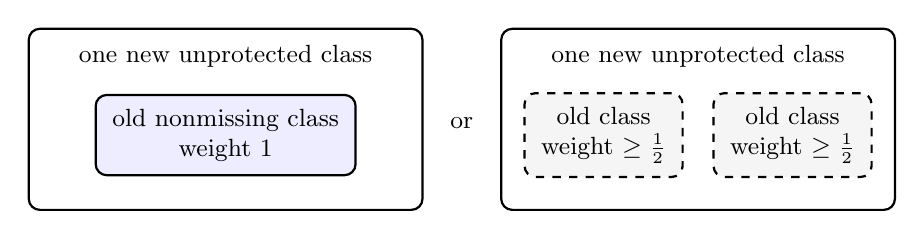
\begin{tikzpicture}[font=\small,thick]
 \draw[rounded corners] (0,0) rectangle (5,2.3);
 \draw[rounded corners] (6,0) rectangle (11,2.3);
 \node at (2.5,1.95) {one new unprotected class};
 \node at (8.5,1.95) {one new unprotected class};
 \node[draw,rounded corners,fill=blue!7,align=center,
       inner xsep=6pt,inner ysep=5pt] at (2.5,0.95)
       {old nonmissing class\\weight $1$};
 \node[draw,dashed,rounded corners,fill=black!4,align=center,
       inner xsep=6pt,inner ysep=5pt] at (7.3,0.95)
       {old class\\weight $\ge\frac12$};
 \node[draw,dashed,rounded corners,fill=black!4,align=center,
       inner xsep=6pt,inner ysep=5pt] at (9.7,0.95)
       {old class\\weight $\ge\frac12$};
 \node at (5.5,1.1) {or};
\end{tikzpicture}
\caption{The weighted containment argument in the chain bound. All
classes shown have one fixed sign and contain no protected label.
Each new class contains either a whole nonmissing old class or two
distinct whole old classes. A missing old class has weight $1/2$;
every other old class has weight $1$. The displayed regions express
set containment schematically. Distinct new classes cannot use the
same whole old class, so their unit weight requirements add.}
\label{fig:nesting-budget}
\end{figure}


By Lemma~\ref{nest:containment}, each unprotected class at stage $j$
contains previous classes of total weight at least $1$:
either one nonmissing class, or two distinct classes.
Every contained previous class is unprotected, since a protected
label in it would also protect the new class.
Distinct new classes cannot use the same previous class, because
classes of a fixed sign are disjoint and the two sign-label sets
are disjoint. Consequently
\[
 s_j\leq s_{j-1}-\frac{\delta_j}{2}.
\]
Summing and using $s_k\geq0$ yields
$\sum_{j=1}^k\delta_j\leq2(s_0-s_k)\leq2|J_0|$.
\end{proof}

\section{An exponential bound for order-reversing images}
\label{amp:section}

We now prove Theorem~\ref{amp:image}, combining transport and the
nested-chain inequality to bound order-reversing relation images.
Write $\mathcal R_H$ for the monoid of all binary relations
on a finite set $H$, with multiplication in path order.  For
$F\subseteq H$, write $I_F=\{(x,x):x\in F\}$; relations on $F$ are
also regarded as relations on $H$ supported on $F\times F$.

The proof amplifies one off-diagonal pair in the image into a family
of pair additions.  The chain inequality bounds their total cost in
missing recurrent classes; restriction to smaller relation monoids
bounds each cost from below.  We first record two elementary facts
that allow these restrictions without losing the hypotheses.
The pattern of relation additions follows the matching-diagram
argument in \cite[Section~3]{CompanionDeterminization2026}; all loss estimates
needed here are supplied by the path-diagram results just proved.

\subsection{Corners and unit lifts}

For an idempotent $d$ in a semigroup $A$, its \emph{corner}
$dAd=\{dad:a\in A\}$ is a monoid with identity $d$.
A \emph{unit} means an element with a two-sided inverse relative to
the specified monoid identity.

\begin{lemma}[Minimal idempotent corners]
\label{amp:minimal-corner}
Let $A$ be a finite semigroup, let $M$ be a monoid, and let
$\theta:A\to M$ be a surjective multiplicative map.  For every
idempotent $q\in M$, there is an idempotent $d\in A$ with
$\theta(d)=q$ that is minimal among such idempotents under
$\trianglelefteq$.  For every such minimal $d$, restriction of
$\theta$ gives a unital surjection
\[
 dAd\longrightarrow qMq.
\]
Every element of $dAd$ whose image is a unit of $qMq$ is itself a
unit of $dAd$.  In particular, every unit of $qMq$ has a unit lift.
\end{lemma}

\begin{proof}
Every element $w$ of a finite semigroup has an idempotent positive
power: the sequence of powers is eventually periodic, so a
sufficiently large exponent divisible by its eventual period gives
$w^{2k}=w^k$.  Applying this to a preimage of $q$ gives an
idempotent preimage of $q$.  Finiteness then gives one minimal in
the nesting order.

For any $y\in qMq$, choose $x\in A$ with $\theta(x)=y$.
Then $\theta(dxd)=qyq=y$, proving surjectivity on the corner;
its identity $d$ maps to $q$.  Now let $w\in dAd$ have unit image.
An idempotent power $w^k$ has an image that is both a unit and an
idempotent in $qMq$, hence equals $q$.  Since
$w^k\trianglelefteq d$, minimality gives $w^k=d$.  If $k>1$,
the element $w^{k-1}$ is a two-sided inverse of $w$ in $dAd$;
if $k=1$, then $w=d$ is already the identity.
\end{proof}

The next lemma identifies a smaller full relation monoid inside an
idempotent corner.  Its hypothesis says that the old relation
restricts to the identity on the retained points.

\begin{lemma}[Restriction of a relation corner]
\label{amp:relation-corner}
Let $P\in\mathcal R_H$ be idempotent, let $F\subseteq H$, and
put $i=I_F$.  Suppose that $iPi=i$, and define $Q=PiP$.
Then $Q$ is idempotent, $Q\trianglelefteq P$, and restriction is
a unital monoid isomorphism
\begin{equation}
 \rho:Q\mathcal R_HQ\longrightarrow\mathcal R_F,
 \qquad \rho(Z)=iZi.
 \label{amp:restriction}
\end{equation}
Its inverse sends $A\in\mathcal R_F$ to $PAP$.
\end{lemma}

\begin{proof}
Using $P^2=P$ and $iPi=i$, we obtain
\[
 Q^2=Q,\qquad PQ=QP=Q,\qquad
 Qi=Pi,\qquad iQ=iP,\qquad iQi=i.
\]
If $Z=QZQ$, then $PZP=Z$, and therefore
\[
 Z=PiPZPiP=PiZiP.
\]
Thus restriction determines $Z$ uniquely.  Conversely, for a
relation $A=iAi$ supported on $F$, the relation $PAP$ belongs to
$Q\mathcal R_HQ$, since $PAP=QAQ$, and
\[
 i(PAP)i=(iPi)A(iPi)=A.
\]
This proves bijectivity with the claimed inverse.  For supported
relations $A,B\in\mathcal R_F$,
\[
 (PAP)(PBP)=PAPBP
           =PA(iPi)BP
           =PABP.
\]
Hence the inverse, and therefore restriction, preserves
multiplication.  Finally $\rho(Q)=i$, the identity of
$\mathcal R_F$.
\end{proof}

\subsection{Amplifying a single added pair}

Set
\begin{equation}
 t=64,\qquad
 D(h)=2^{\lfloor(h-2)/(2t-1)\rfloor}\quad(h\geq2).
 \label{amp:D}
\end{equation}
The choice $t=64$ balances the two estimates proved below: $t^2$
pair additions each cost at least half the smaller-instance bound,
while their total cost is at most $16t$ times the original loss.
The resulting gain is $t/32=2$, at a reduction of $2t-1=127$ points.
We prove a missing-set bound strong enough to survive passage to
any of the corners above.  The additional unit-lifting hypothesis
permits conjugation by arbitrary permutations of $H$; Lemma
\ref{amp:minimal-corner} will supply it when we return to Theorem
\ref{amp:image}.

\begin{proposition}[Cost of one added pair]
\label{amp:single-edge}
Let $m\geq1$, let $e\in\mathcal T_m$ be idempotent, and let
$S\subseteq e\mathcal T_me$ be a submonoid with identity $e$.
Let $H$ be a finite set of cardinality $h\geq2$.  Suppose that
$\phi:S\to\mathcal R_H$ is a unital surjective homomorphism
such that
\[
 z\sqsubseteq w\ \Longrightarrow\ \phi(w)\subseteq\phi(z)
 \qquad(z,w\in S),
\]
and suppose that each permutation of $H$ has a lift that is a
unit of $S$.  If $a\in S$ is idempotent and, for distinct $x,y\in H$,
\[
 \phi(a)=I_H\cup\{(x,y)\},
\]
then $|\mathcal M_e(a)|\geq D(h)$.
\end{proposition}

\begin{proof}
We induct on $h$, simultaneously over all the data in the
statement, including $m$, $e$, $S$, and $\phi$.
For $2\leq h\leq2t$, we have $D(h)=1$.
If $\mathcal M_e(a)$ were empty, Lemma
\ref{diag:rectangles} would give $e\sqsubseteq a$.
Order reversal would then give
$I_H\cup\{(x,y)\}\subseteq I_H$, a contradiction.

Assume henceforth that $h\geq2t+1$, and put
$c=|\mathcal M_e(a)|$.  We will construct $t^2$ nested steps
with total missing-set size at most $16tc$.  Each step will
contain a smaller instance of the Proposition, on $h-2t+1$
points.

\medskip
\noindent\textbf{Step 1: A common budget for all pair additions.}
Choose disjoint sets
\[
 U=\{u_1,\ldots,u_t\},\qquad
 V=\{v_1,\ldots,v_t\},\qquad \{z\}
\]
in $H$.  Conjugating $a$ by unit lifts of permutations gives
elements $s_i,s'_j\in S$ with
\begin{equation}
 \phi(s_i)=I_H\cup\{(u_i,z)\},\qquad
 \phi(s'_j)=I_H\cup\{(z,v_j)\}.
 \label{amp:hub}
\end{equation}
Indeed, permutation conjugation acts transitively on ordered
pairs of distinct points, and the inverse of a unit lift maps
to the inverse permutation.  Explicitly, a unit $p\in S$
gives the conjugate $pap^{-1}$, with $pep^{-1}=e$.
Applying Lemma \ref{diag:transport} with
$J=\mathcal M_e(a)$ therefore gives
\[
 |\mathcal M_e(s_i)|\leq2c,\qquad
 |\mathcal M_e(s'_j)|\leq2c.
\]
Consequently the single set
\[
 J=\bigcup_{i=1}^t\mathcal M_e(s_i)
       \ \cup\ \bigcup_{j=1}^t\mathcal M_e(s'_j)
       \ \subseteq\mathcal C_e
\]
has $|J|\leq4tc$, and the product inequality of Lemma
\ref{diag:missing} gives
$\mathcal M_e(s_i s'_j)\subseteq J$ for every $i,j$.

Let $P_0=I_{H\setminus\{z\}}$.  Choose an idempotent lift
$b_0\in S$ of $P_0$, by taking an idempotent positive power
of any lift, and define
\[
 g_{ij}=b_0s_i s'_j b_0\in b_0Sb_0.
\]
The image of $s_i s'_j$ consists of the identity and the three
pairs $(u_i,z)$, $(z,v_j)$, and $(u_i,v_j)$.
The outer factors $P_0$ remove the first two, so
\begin{equation}
 \phi(g_{ij})=P_0\cup\{(u_i,v_j)\}.
 \label{amp:pair-image}
\end{equation}
Figure~\ref{fig:hub} illustrates this conversion of two generator
families into a family indexed by $U\times V$.

\begin{figure}[htbp]
\centering
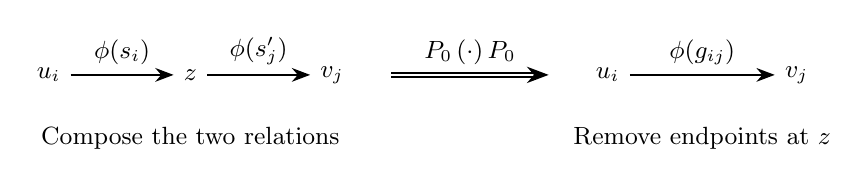
\begin{tikzpicture}[>=Stealth,font=\small,thick]
 \node (u) at (0,0) {$u_i$};
 \node (z) at (1.8,0) {$z$};
 \node (v) at (3.6,0) {$v_j$};
 \draw[->] (u)--node[above] {$\phi(s_i)$}(z);
 \draw[->] (z)--node[above] {$\phi(s'_j)$}(v);
 \node[align=center] at (1.8,-0.8) {Compose the two relations};
 \draw[->,double] (4.35,0)--node[above] {$P_0\,(\cdot)\,P_0$}(6.35,0);
 \node (uu) at (7.1,0) {$u_i$};
 \node (vv) at (9.5,0) {$v_j$};
 \draw[->] (uu)--node[above] {$\phi(g_{ij})$}(vv);
 \node[align=center] at (8.3,-0.8) {Remove endpoints at $z$};
\end{tikzpicture}
\caption{The relation images of the hub construction, with identity
pairs omitted. Composing the $u_i\to z$ and $z\to v_j$ additions
creates $u_i\to v_j$; sandwiching by $P_0$ removes the two pairs
incident to $z$. The $2t$ generators yield all $t^2$ pair additions.}
\label{fig:hub}
\end{figure}


Since $b_0eb_0=b_0$, the common-set conclusion of Lemma
\ref{diag:transport} gives a \emph{single} set
$J_0\subseteq\mathcal C_{b_0}$ such that
\begin{equation}
 |J_0|\leq8tc,\qquad
 \mathcal M_{b_0}(g_{ij})\subseteq J_0
 \quad(1\leq i,j\leq t).
 \label{amp:common-budget}
\end{equation}

\medskip
\noindent\textbf{Step 2: A nested chain spending that budget.}
List the $t^2$ pairs of $U\times V$ in any order, without
repetitions.  Let $E_\ell$ be the set of the first $\ell$
pairs, and put $P_\ell=P_0\cup E_\ell$ for
$0\leq\ell\leq t^2$.  For any $E,E'\subseteq U\times V$,
\begin{equation}
 (P_0\cup E)(P_0\cup E')=P_0\cup E\cup E'.
 \label{amp:union}
\end{equation}
To check this, $P_0$ acts as the identity on all the endpoints
in question, and no pair of $E$ can be followed by a pair of
$E'$, because $U\cap V=\varnothing$.
In particular, every $P_\ell$ is idempotent.

If the pair at position $\ell$ is $(u_i,v_j)$, choose
$b_\ell$ to be an idempotent positive power of
$b_{\ell-1}g_{ij}b_{\ell-1}$.
Inductively, Equation \eqref{amp:union} gives
$\phi(b_\ell)=P_\ell$.
The sandwich, and hence all its positive powers, is absorbed
on both sides by $b_{\ell-1}$.  Thus
\[
 b_\ell\trianglelefteq b_{\ell-1}
 \qquad(1\leq\ell\leq t^2).
\]
All these elements lie in the $b_0$-corner.  Starting with
$\mathcal M_{b_0}(b_0)=\varnothing$, repeated use of Lemma
\ref{diag:missing} and Equation \eqref{amp:common-budget}
shows that
\[
 \mathcal M_{b_0}(b_\ell)\subseteq J_0
 \qquad(0\leq\ell\leq t^2).
\]
Here taking a positive power cannot enlarge the missing set:
all factors have the same missing set, and their union is
unchanged.  Proposition \ref{nest:chain} now yields
\begin{equation}
 \sum_{\ell=1}^{t^2}\delta_\ell\leq16tc,
 \qquad
 \delta_\ell=|\mathcal M_{b_{\ell-1}}(b_\ell)|.
 \label{amp:total-cost}
\end{equation}
We have bounded the total cost of the chain using only the
$2t$ original conjugates.  It remains to give an inductive
lower bound for each of its $t^2$ steps.

\medskip
\noindent\textbf{Step 3: A smaller instance inside every step.}
Fix $\ell$, let $(u_i,v_j)$ be its newly added pair, and
write $b=b_{\ell-1}$ and $P=P_{\ell-1}$.  Retain the two
endpoints of this pair and all points outside the construction:
\[
 F=\{u_i,v_j\}\cup
       \bigl(H\setminus(U\cup V\cup\{z\})\bigr),
 \qquad i_F=I_F,\qquad Q=Pi_FP.
\]
Then $|F|=h-2t+1\geq2$.  Among the possible extra pairs
of $P$, only $(u_i,v_j)$ has both endpoints in $F$, and this
pair has not yet been added.  Therefore
$i_FPi_F=i_F$.  By Lemma \ref{amp:relation-corner},
$Q\trianglelefteq P$ and restriction gives
$Q\mathcal R_HQ\simeq\mathcal R_F$.
Moreover, Equation \eqref{amp:union} gives
$PP_\ell P=P_\ell$.  Using $i_FQ=i_FP$ and
$Qi_F=Pi_F$, we obtain
\begin{equation}
 i_F(QP_\ell Q)i_F
 =i_FP_\ell i_F
 =I_F\cup\{(u_i,v_j)\}.
 \label{amp:compressed-pair}
\end{equation}

Consider the finite monoid $A=bSb$.  The restriction of
$\phi$ maps it onto $P\mathcal R_HP$: sandwiching any
preimage by $b$ gives a preimage of its $P$-sandwich.
Apply Lemma \ref{amp:minimal-corner} \emph{inside $A$} to
the idempotent $Q$.  We obtain an idempotent $d\in A$ with
$\phi(d)=Q$, minimal there among idempotent lifts of $Q$.
Its corner $dAd$ maps unitally onto
\[
 Q(P\mathcal R_HP)Q=Q\mathcal R_HQ,
\]
and all units of this image have unit lifts.  Composing with
restriction gives a unital surjective homomorphism
\begin{equation}
 \psi:dAd\longrightarrow\mathcal R_F,
 \qquad \psi(w)=i_F\phi(w)i_F.
 \label{amp:smaller-map}
\end{equation}
This map is order-reversing because $\phi$ is and restriction
preserves inclusion.  It has unit lifts of every permutation
of $F$, by the isomorphism in Lemma
\ref{amp:relation-corner}.  Also $dAd$ is a submonoid of
$d\mathcal T_md$ with identity $d$.
These observations verify all the map and domain hypotheses
needed for induction.

Because $b_\ell\trianglelefteq b$, we have $b_\ell\in A$.
By Equation \eqref{amp:compressed-pair}, the element
$db_\ell d\in dAd$ maps under $\psi$ to
$I_F\cup\{(u_i,v_j)\}$.  This relation is idempotent, so
an idempotent positive power $v$ of $db_\ell d$ has the same
image.  Since $d\in A$ is idempotent, $dbd=d$.
Apply Lemma \ref{diag:transport} from the identity $b$ to
the identity $d$, with context $(d,d)$ and missing set
$\mathcal M_b(b_\ell)$.  Then apply the power consequence
of Lemma \ref{diag:missing} in the $d$-corner.  This gives
\begin{equation}
 |\mathcal M_d(v)|
 \leq |\mathcal M_d(db_\ell d)|
 \leq 2\delta_\ell.
 \label{amp:step-cost}
\end{equation}
The induction hypothesis applies to $d$, $dAd$, $\psi$,
and $v$, with the smaller parameter $|F|=h-2t+1$.
It follows that
\[
 2\delta_\ell\geq D(h-2t+1).
\]

Summing this lower bound and using Equation
\eqref{amp:total-cost}, we conclude that
\[
 16tc\ \geq\ \frac{t^2}{2}D(h-2t+1),
 \qquad
 c\ \geq\ \frac{t}{32}D(h-2t+1).
\]
For $t=64$, the last expression is
$2D(h-127)=D(h)$, by the definition of $D$.
This completes the induction.
\end{proof}

\begin{proof}[Proof of Theorem \ref{amp:image}]
Apply Lemma \ref{amp:minimal-corner} to $\phi_0$ and the
idempotent $I_H$.  It supplies an idempotent $e\in S_0$
such that $S=eS_0e$ maps unitally onto $\mathcal R_H$ and
every permutation has a unit lift.  The restricted map
retains order reversal, and $S$ is a submonoid of
$e\mathcal T_me$ with identity $e$.

Choose distinct $x,y\in H$ and any lift in $S$ of
$I_H\cup\{(x,y)\}$.  An idempotent positive power $a$
of that lift has the same image.  Proposition
\ref{amp:single-edge} therefore gives
\[
 D(h)\leq|\mathcal M_e(a)|\leq|\mathcal C_e|\leq2m,
\]
as required.
\end{proof}

\section{Finite computations and the main lower bound}\label{auto:section}

We complete the concrete obligations deferred in
Section~\ref{sec:diagrams}: constructing the small source automaton and
proving the finite-computation representation. The order-reversing map
has already been derived in Proposition~\ref{auto:order-reversal};
we then combine it with Theorem~\ref{amp:image} to finish the main proof.
Throughout, we use the automaton model fixed in the introduction,
including stay moves, finite acceptance, and acceptance in the initial
configuration.

\subsection{The source automaton}

Fix a set $H$ of size $h\geq2$. Recall that the alphabet is
$\Sigma_H=\mathcal R_H$, the word product is $r(w)$ with
$r(\varepsilon)=I_H$, and
\begin{equation}\label{auto:language}
 L_H=\{w\in\Sigma_H^*:r(w)\ne\varnothing\}.
\end{equation}

\begin{lemma}\label{auto:source}
The language $L_H$ is recognized by a 2NFA with exactly $h+2$ states.
\end{lemma}
\begin{proof}
Use one initial state $q_{\mathrm{in}}$, the $h$ states in $H$, and one
accepting state $q_{\mathrm{acc}}$, all distinct.  From
$q_{\mathrm{in}}$ on the left endmarker, the machine moves right into any
chosen state of $H$.  On a letter $R\in\mathcal R_H$, it may move right
from $p\in H$ to $q\in H$ precisely when $(p,q)\in R$.  At the right
endmarker, every state in $H$ has a stay transition to
$q_{\mathrm{acc}}$.  There are no other transitions, and
$q_{\mathrm{acc}}$ is the only accepting state.

On $R_1\cdots R_k$, an accepting computation is exactly a sequence
$p_0,\ldots,p_k\in H$ with $(p_{i-1},p_i)\in R_i$ for
$1\leq i\leq k$.  Such a sequence exists exactly when the relation
product is nonempty.  For $k=0$, the initial move reaches the right
endmarker directly, and the machine accepts.  This agrees with
$r(\varepsilon)=I_H\ne\varnothing$.
\end{proof}

\subsection{Finite computations as diagram paths}
\label{auto:finite-computations}

We now prove the representation promised in
Lemma~\ref{auto:representation}. The construction records arbitrary
finite computations, including stay moves and repeated crossings of the
same cut. It does not require termination of every computation.

\begin{proof}[Proof of Lemma~\ref{auto:representation}]
Let $B$ be the $s$-state automaton in the lemma, with state set $Q$ and
initial state $q_0$. Introduce
one new state $q_\dagger$.  From every original accepting state, at
every cell, add a stay transition to $q_\dagger$.  In state
$q_\dagger$, move right regardless of the scanned symbol, finally
exiting past the right endmarker in state $q_\dagger$.  This last exit
is only a device for representing acceptance, not a transition of the
original machine.  All original transitions remain subject to the
endmarker restrictions.

A finite augmented computation from the original initial configuration
to the designated exit exists if and only if $B$ accepts.  Indeed, an
accepting original computation can be followed by the added stay and
rightward sweep.  Conversely, the first entry into $q_\dagger$ must
come from an original accepting configuration.  This argument includes
the case that $q_0$ itself is accepting.  Infinite computations create
no additional finite successful computation.

Put $\widehat Q=Q\cup\{q_\dagger\}$ and $m=s+1$.  Take the
directional label sets to be two disjoint copies
\[
  D^+=\{q^+:q\in\widehat Q\},
  \qquad
  D^-=\{q^-:q\in\widehat Q\}.
\]
For a cell symbol $c$, including either endmarker with its boundary
rules, let $E_c$ be the relation on $\widehat Q$ given by the augmented
stay transitions.  Let $T_c^+$ and $T_c^-$ be the relations given by
the augmented rightward and leftward transitions, respectively; their second
coordinates record the state \emph{after} the move.  At the right
endmarker, $T_c^+$ includes only the designated augmented exit, and at
the left endmarker $T_c^-$ is empty.  Define a diagram $d_c$ by
\begin{align*}
 (q^+,p^+)\in F_{d_c}
 &\quad\Longleftrightarrow\quad
 (q^-,p^+)\in R_{d_c}
 \quad\Longleftrightarrow\quad
 (q,p)\in E_c^*T_c^+,\\
 (q^-,p^-)\in B_{d_c}
 &\quad\Longleftrightarrow\quad
 (q^+,p^-)\in L_{d_c}
 \quad\Longleftrightarrow\quad
 (q,p)\in E_c^*T_c^-.
\end{align*}
Thus each local diagram edge represents a finite sequence of stays,
possibly empty, followed by one move out of the cell.  The incoming
sign specifies the side of entry, not additional machine memory; the
transition rules themselves depend only on the state and symbol.

Set $\lambda=d_{\mathrm{left}}$ and
$\rho=d_{\mathrm{right}}$ for the two endmarkers, and set
\[
  \tau(c_1\cdots c_k)=d_{c_1}\cdots d_{c_k},
  \qquad \tau(\varepsilon)=1_{\mathcal T_m}.
\]
This is a monoid homomorphism.  Every finite augmented computation
ending in the designated exit decomposes into successive visits to
individual cells, each consisting of finitely many stays and one
exit move.  These visits give a path through the product of the cell
diagrams.  In the opposite direction, each local edge in a finite
diagram path has a finite transition witness.  Expanding these
witnesses and concatenating them gives an augmented computation,
because the exit state from one cell is exactly the entry state to
the next.  Neither direction assumes that a cut is crossed at most
once.

The fictitious entry into the left endmarker with label $q_0^+$
represents the initial configuration; it is not an additional machine
transition.  No path can leave the tape to the left, and a path can
leave to the right only through the designated exit.  Hence
\eqref{auto:recognition} holds with $a=q_0^+$ and $b=q_\dagger^+$.
For the empty word, the two endmarker cells are adjacent, and the
identity $\tau(\varepsilon)$ gives precisely their product.  A stay
cycle causes no difficulty: only its finite traversals are represented
in $E_c^*$.
\end{proof}

\begin{remark}[Other standard conventions]\label{auto:conventions}
The exponential conclusion also survives the usual changes of starting
position or acceptance convention, with possible changes to the additive
state offsets. To use our representation for a machine whose convention
requires a positive transition into an accepting state, add a fresh
nonaccepting initial copy with the same outgoing transitions, keeping all original states and
transition destinations. This prevents the initial configuration alone
from accepting, while preserving every acceptance after a transition.
Starting on the first input cell can be simulated from the left
endmarker by one additional initial state. If success must occur at a designated marker or on a specified
exit, enable the added success routine only at that local accepting
event. These versions of the path representation use $m=s+O(1)$ labels
per sign, and the source automaton still uses $h+O(1)$ states. The exact
offsets in Theorem~\ref{main:theorem} refer to the convention fixed in
the introduction.
\end{remark}

\begin{proof}[Proof of Theorem~\ref{main:theorem}]
For any $n\geq4$, let $h=n-2$, choose a set $H$ of size $h$, and use
the $n$-state source automaton from Lemma~\ref{auto:source}.
If an $s$-state 2NFA recognizes its complement, then
Proposition~\ref{auto:order-reversal} supplies the order-reversing
relation image required by Theorem~\ref{amp:image}.  With $m=s+1$,
that bound gives
\[
  2(s+1)\geq 2^{\lfloor(h-2)/127\rfloor}
            =2^{\lfloor(n-4)/127\rfloor}.
\]
Rearranging proves the stated lower bound.  Since its right-hand side
grows exponentially with $n$, no fixed polynomial can bound the
complementation cost for all finite alphabets.
\end{proof}

\subsection{The determinization consequence}

The lower bound also applies indirectly to deterministic simulation.
Here we use one external automata transformation: deterministic two-way
automata can be complemented with linear state overhead independent of
the alphabet, even when the original computation may fail to halt
\cite{GeffertMereghettiPighizzini2007}. The possible nonaccepting loops
are the reason that exchanging accepting and rejecting states alone
does not give this transformation.

\begin{corollary}\label{auto:determinization}
There are absolute constants $c>0$ and $n_0$ such that, for every
$n\ge n_0$, every 2DFA recognizing the language of the $n$-state 2NFA
$A_n$ in Theorem~\ref{main:theorem} has at least
\[
 c\,2^{\lfloor(n-4)/127\rfloor}
\]
states. Hence no polynomial state bound independent of the finite
alphabet can determinize all 2NFAs.
\end{corollary}
\begin{proof}
We use only the linear-overhead conclusion of
\cite{GeffertMereghettiPighizzini2007}, allowing constant-factor changes
for model conventions. The standard marker model and its normalization
are described in the precursor \cite[Section~2 and Lemma~3.1]{GeffertMereghettiPighizzini2005}.
Stay moves can be replaced by a two-step
excursion that stores the destination state and the return direction
in a fixed number of copies of the state set. The excursion goes left
at the right endmarker and right elsewhere. Even on the empty word,
the two distinct endmarker cells provide the needed adjacent cell.
Auxiliary states are nonaccepting, and the destination state is entered
only on returning to the original cell. A reached accepting
configuration, including the initial configuration, can instead start
a fixed marker sweep to a designated accepting halt. Missing
transitions can halt and reject. These changes require $O(s+1)$ states
for an $s$-state 2DFA and preserve finite acceptance. The cited
transformation supplies the substantive additional step of handling
infinite nonaccepting computations.

Thus an $s$-state deterministic recognizer for $L(A_n)$ has a
deterministic complement, also a 2NFA, with at most $C(s+1)$ states
for an absolute constant $C$. Theorem~\ref{main:theorem} gives
\[
 C(s+1)\ge \tfrac12\,2^{\lfloor(n-4)/127\rfloor}-1.
\]
For all sufficiently large $n$ this implies the asserted bound with
an absolute $c>0$. Since the same alphabets are finite for every $n$,
it also excludes every polynomial bound uniform over alphabets.
\end{proof}

For comparison, the companion theorem
\cite[Theorem~1.1]{CompanionDeterminization2026} gives
\[
 4(s+2)^2\geq 2^{\lfloor(h-2)/31\rfloor}
\]
for an $s$-state deterministic recognizer of the same language $L_H$.
That theorem also states the improvement from $s+2$ to $s+1$ when the
initial configuration counts as acceptance, as it does here. Its
exponent therefore grows as $h/62$, compared with $h/127$ in
Corollary~\ref{auto:determinization}. The source constructions use
$h+3$ and $h+2$ states, respectively: the companion includes a rejecting
sink, which the partial source automaton above does not need. Its
matching-diagram proof gives a stronger deterministic bound independently
of the complementation theorem proved here.

{\raggedright
\bibliographystyle{plain}
\bibliography{references}
}
\end{document}
